%!TEX root = ../thesis.tex

\section{問題}
我々が行ってきた研究では, 簡易的なシミュレータ上で提案手法が有効だと確認されている. そのため, 前章では次の段階として, 実環境における提案手法の有効性を検証することを試みた. しかし, 学習時間の長さが問題となり, 評価を十分な回数行うことができなかった. そのため, 学習時間の短縮が必要であると判断した. 2つのアプローチを提案し, 学習量の削減を図る.

% \begin{itemize}
%   \item 実験条件(主にカメラ画像に影響を及ぼす光である)を揃える関係上, 実験を行う時間帯を光の変化が少ない夜間に固定する必要があるため, 1日に実験を行える時間が少なく, 1回の学習に何日も費やす必要がある
%   \item 長時間の学習に耐えられるだけのバッテリ容量がロボットにない
% \end{itemize}

% これらの課題点から, 
% \par
% この節では, まず, 従来の実験を簡単に紹介する. 次に, 2つのアプローチについての詳細と行った実験を述べる. 最後に, アプローチを試みる前と各アプローチによる実験結果を比較し, 議論を行う.

\newpage
\section{単に学習量を減らした実験}

% \begin{itemize}
%   \item 実験目的\\
%   簡易的なシミュレータ上で, 提案手法の有効性の検証を行う
%   \item 実験装置\\
%   4.1.1で述べた簡易的なシミュレータ環境とロボットで実験を行った
%   \item 実験方法\\
%   4.1.2で示した経路を繰り返し走行させる. 学習を60000step実行後, テストフェーズに移行する. テストフェーズで正しい順序で経路を選択し, 走行を行えるか確認する. この一連の流れを10回繰り返し行う.

%   \newpage

%   \item 実験結果\\
%   実験結果を\figref{Fig:60000step}に示す. この図は, それぞれの走行パターンにおいて正しく経路を選択し, 走行できた回数を表している. \tabref{table:result}に全パターンの成功回数を合計した結果を示す. なお, 分母が120であるのはテストフェーズにおいて, 全12パターンからなる経路を走行させ, 評価を行うことを10回繰り返したためである. 
%   \par
%   \tabref{table:result}に示すように, 目標方向に従って113/120回, 正しい経路を選択する様子が見られた. 

% \vspace{1cm}

% \begin{figure}[hbtp]
%   \centering
%  \includegraphics[keepaspectratio, scale=0.5]
%       {images/60000step.png}
%  \caption{Experimental results for each moving pattern from \cite{mech}}
%  \label{Fig:60000step}
% \end{figure}

% \vspace{1cm}

% \begin{table}[hbtp]
%   \caption{Experimental results}
%   \label{table:result}
%   \centering
%   \begin{tabular}{|c|c|c|}
%     \hline
%     Experiments & Step & Total result\\
%     \hline
%     Conventional & 60000 & 113/120(94.2\%)\\
%     \hline
%   \end{tabular}
% \end{table}

% \end{itemize}

% \newpage

前章のシミュレータ上での実験を基に, 単に60000stepから10000stepに学習量を変更し, 実験した結果を下記に示す.

実験結果を \figref{Fig:10000step} に示す. この図は, それぞれの走行パターンにおいて正しく経路を選択し, 走行できた回数を表している. \tabref{table:result_without} に実験ごとに全パターンの成功回数を合計した結果を示す. \tabref{table:result_without} に示すように, 目標方向に従って 87/120 回, 正しい経路を選択する様子が見られた.

60000stepの実験と成功率を比較すると約22\%ほどの差がある. これでは, 学習量を削減できたとは言い難い. そのため, 後述する2つのアプローチを試みることで成功率の改善を図る.

\vspace{0.5cm}

\begin{figure}[hbtp]
  \centering
 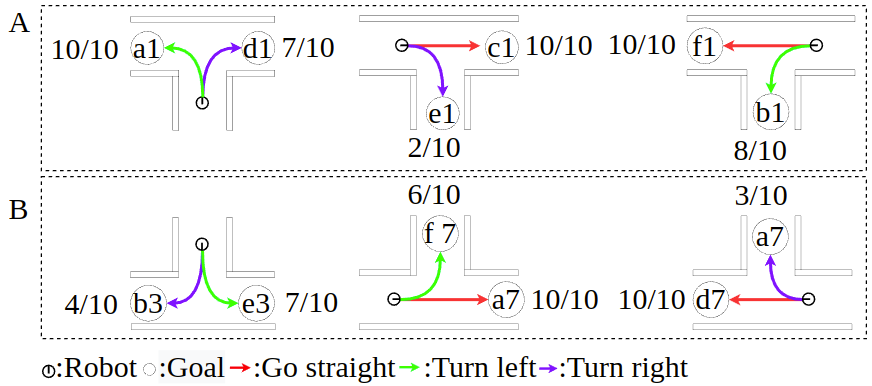
\includegraphics[keepaspectratio, scale=0.43]
      {images/10000step.png}
 \caption{Experimental results for each moving pattern at 10000step by conventional}
 \label{Fig:10000step}
\end{figure}  

\vspace{0.5cm}

\begin{table}[hbtp]
  \caption{Experimental results at 10000step by conventional}
  \label{table:result_without}
  \centering
  \begin{tabular}{|c|c|c|}
    \hline
    Experiments & Step & Total results\\
    \hline
    Conventional & 60000 & 113/120(94.2\%)\\
    \hline
    Conventional & 10000 & 87/120(72.5\%)\\
    \hline
  \end{tabular}
\end{table}

\newpage



\section{アプローチ1:データセットに加えるデータの割合変更}
従来の実験における10000stepごとのコマンドに対応するデータ数を\figref{Fig:hist}に示す. \figref{Fig:hist} (a)より, 直進コマンド時のデータ数が圧倒的に多いことがわかる. このデータ数の偏りを解消するため, \figref{Fig:hist} (b)に示すように, 左折と右折コマンドのデータ数を7倍にする. 7倍にするのは, 左折と右折コマンドのデータ数を直進コマンドと同程度にするためである. なお, データ数を何倍にするのが望ましいのか本論文では議論しない. 実験により, データセットに加えるデータ数の割合変更が有効か検証する.

% \begin{figure}[h]
%   \begin{minipage}[b]{0.5\linewidth}
%     \centering
%  \includegraphics[keepaspectratio, scale=0.3]
%       {images/hist_change_org.png}
%  \subcaption{hoge}
%  \label{Fig:hist_org}
% %  \label{Fig:hist_change_org}
% \end{minipage}

%   \begin{minipage}[b]{0.5\linewidth}
%     \centering
%  \includegraphics[keepaspectratio, scale=0.3]
%       {images/hist_change_times7.png}
%  \subcaption{jkofs}
%  \label{Fig:hist_times7}
% %  \label{Fig:hist_change_times7}
%   \end{minipage}
%   \caption{Number of data per command per 10000steps in conventional experiments}
%    \label{Fig:hist}
% \end{figure}

\begin{figure}[h]
  \centering
  \begin{minipage}[b]{67mm}
    \centering
    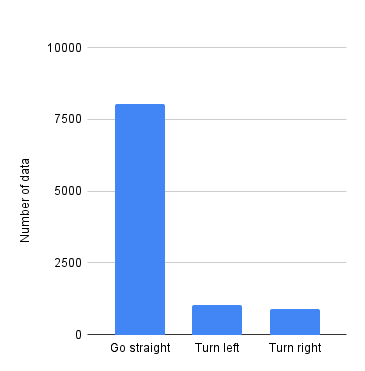
\includegraphics[width=67mm]{images/hist_change_org.png}
    \caption*{(a)}
  \end{minipage} 
  % \newpage
  % \hspace{0.03\columnwidth}
  \begin{minipage}[b]{67mm}
    \centering
    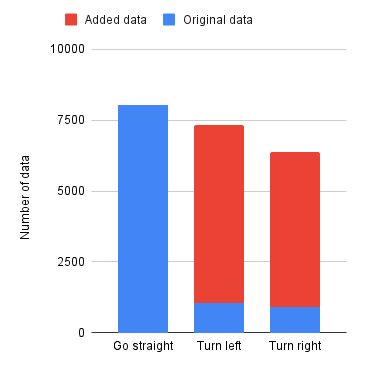
\includegraphics[width=67mm]{images/hist_change_times7.png}
    \caption*{(b)}
  \end{minipage}
  \caption{Number of data per command per 10000steps in conventional experiments}
  \label{Fig:hist}
\end{figure}

% \begin{itemize}
  \subsection{実験目的}
  データセットに加えるデータの割合変更が有効か検証を行う
  \subsection{実験装置}
  4.2で述べた簡易的なシミュレータ環境とロボットで実験を行った
  \subsection{実験方法}
  4.3で示した経路を繰り返し走行させる. 学習を10000step実行後, テストフェーズに移行する. テストフェーズで正しい順序で経路を選択し, 走行を行えるか確認する. この一連の流れを10回繰り返し行う.
  % \newpage
  \subsection{実験結果}
  実験結果を\figref{Fig:10000step_act1.0}に示す. この図は, それぞれの走行パターンにおいて正しく経路を選択し, 走行できた回数を表している. \tabref{table:result3}に実験ごとに全パターンの成功回数を合計した結果を示す. 
  \tabref{table:result3}に示すように, 目標方向に従って99/120回, 正しい経路を選択する様子が見られた. 
  \par
  60000stepの実験と成功率を比較すると約12\%ほど差があり, アプローチ1を試みた結果では成功率が十分だとは言い難い. 次に成功率を改善するため, 後述するアプローチ2を試みた.

  % \vspace{0.5cm}

  \begin{figure}[hbtp]
    \centering
   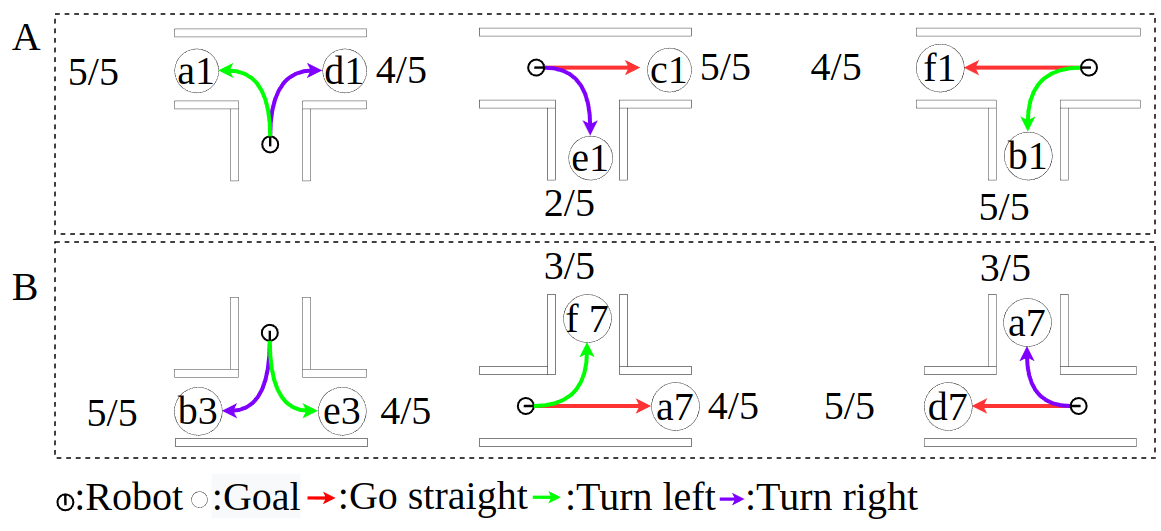
\includegraphics[keepaspectratio, scale=0.4]
        {images/10000step_act1.0.png}
   \caption{Experimental results for each moving pattern by Approach1}
   \label{Fig:10000step_act1.0}
  \end{figure}  
  
  % \vspace{0.5cm}

  \begin{table}[hbtp]
    \caption{Experimental results by Approach 1}
    \label{table:result3}
    \centering
    \begin{tabular}{|c|c|c|}
      \hline
      Experiments & Step & Total results\\
      \hline
      Conventional & 60000 & 113/120(94.2\%)\\
      \hline
      Conventional & 10000 & 87/120(72.5\%)\\
      \hline
      Approach1:percentage change of data & 10000 & 99/120(82.5\%)\\
      \hline
    \end{tabular}
  \end{table}

% \end{itemize}

\newpage

\newpage

\section{アプローチ2:学習フェーズにおける積極的な蛇行}
清岡ら\cite{kiyooka}により, 目標経路上に加えて離れた状態を学習することが, テストフェーズでの走行に大きな影響を与えるため, 重要だとされている. そのため, より積極的に蛇行を行い, 目標経路から離れた状態を増加させることを検討する. \par
実験で用いているシステムの学習フェーズでは,  \figref{Fig:act1.0}に示すようにロボットが目標経路上付近を走行している場合, 訓練中の学習器へ画像を入力し, 出力される角速度を用いて走行している. この場合に, 目標経路から一定の距離離れると地図を用いたルールベース制御器の走行に切り替わり, 強制的にロボットを目標経路上に戻すように制御を行う. 

\begin{figure}[hbtp]
  \centering
 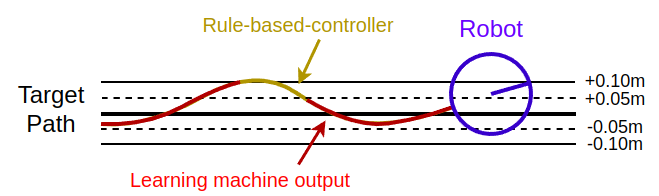
\includegraphics[keepaspectratio, scale=0.58]
      {images/act1.0.png}
 \caption{Moving on the target path}
 \label{Fig:act1.0}
\end{figure}

訓練中の学習器へ画像を入力し, \figref{Fig:3action}のように出力される角速度を1.5倍にする. その結果, \figref{Fig:act1.5}に示すように蛇行する頻度が高くなり, 目標経路から離れた状態をより多く学習できる可能性がある. なお, 得られた角速度を何倍にするのが望ましいのか本論文では議論しない. 実験により, 学習フェーズにおける積極的な蛇行が有効か検証する.

\begin{figure}[hbtp]
  \centering
 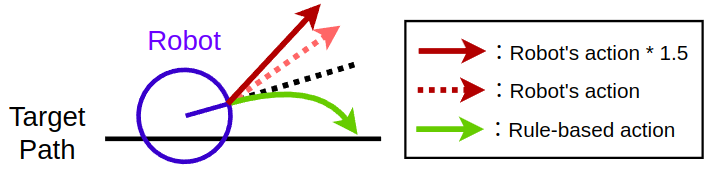
\includegraphics[keepaspectratio, scale=0.5]
      {images/3action2.png}
 \caption{Robot behavior}
 \label{Fig:3action}
\end{figure}

\begin{figure}[hbtp]
  \centering
 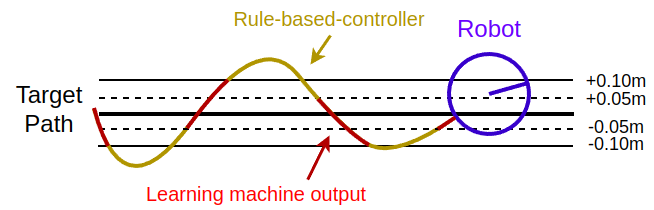
\includegraphics[keepaspectratio, scale=0.58]
      {images/act1.5.png}
 \caption{Moving on the target path attempting approach 2}
 \label{Fig:act1.5}
\end{figure}

% \vspace{-1cm}

% \begin{itemize}
  \subsection{実験目的}
  学習フェーズにおける積極的な蛇行が有効か検証を行う
  \subsection{実験装置}
  4.2で述べた簡易的なシミュレータ環境とロボットで実験を行った
  \subsection{実験方法}
  4.3で示した経路を繰り返し走行させる. 学習を10000step実行後, テストフェーズに
  移行する. テストフェーズで正しい順序で経路を選択し, 走行を行えるか確認する. こ
  の一連の流れを10回繰り返し行う.
  \subsection{実験結果}
  実験結果を\figref{Fig:10000step_act1.5}に示す. この図は, それぞれの走行パターンにおいて正しく経路を選択し, 走行できた回数を表している. \tabref{table:result4}に実験ごとに全パターンの成功回数を合計した結果を示す. 
  \tabref{table:result4}に示すように, 目標方向に従って109/120回, 正しい経路を選択する様子が見られた. 
  % また, 
  % \par
  % \tabref{table:result4}からアプローチ1の実験より, 成功率が改善していることがわかる. また, 60000stepの実験と成功率を比較した場合, 約4\%ほどの差がある. これには, 以下2つの要因が挙げられる.
  % \begin{itemize}
  %   \item 
  % \end{itemize}
  % そのため, 10000stepから20000stepに学習量を増加し, 実験した結果を下記に示す.

  
  \begin{figure}[hbtp]
    \centering
   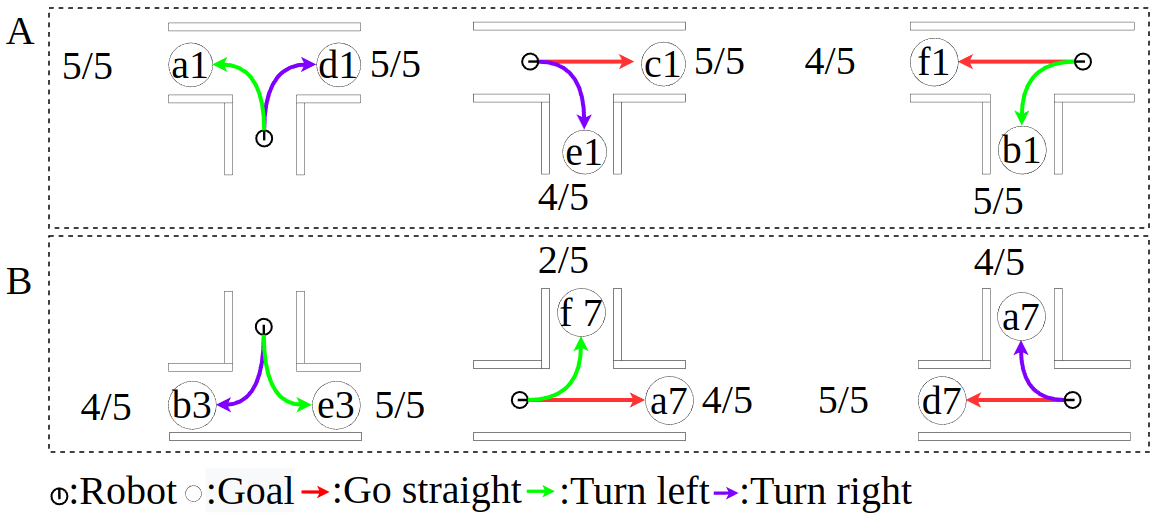
\includegraphics[keepaspectratio, scale=0.55]
        {images/10000step_act1.5.png}
   \caption{Experimental results for each moving pattern at 10000step by Approach 1+2}
   \label{Fig:10000step_act1.5}
  \end{figure}  
  
  % \vspace{0.5cm}

  \begin{table}[hbtp]
    \caption{Experimental results at 10000step by Approach 1+2}
    \label{table:result4}
    \centering
    \begin{tabular}{|c|c|c|}
      \hline
      Experiments & Step & Total results\\
      \hline
      Conventional & 60000 & 113/120(94.2\%)\\
      \hline
      Conventional & 10000 & 87/120(72.5\%)\\
      \hline
      Approach1:percentage change of data & 10000 & 99/120(82.5\%)\\
      \hline
      \begin{tabular}{c}
        \textbf{Approach1:percentage change of data}\\
        % \textbf{+}
        \textbf{+ Approach2:aggressive meandering}
      \end{tabular}
       & \textbf{10000} & \textbf{109/120(90.8\%)}\\
      \hline
    \end{tabular}
  \end{table}

  % \vspace{1cm}

  \tabref{table:result4}からアプローチ1の実験より, 成功率が改善していることがわかる. また, 60000stepの実験と成功率を比較した場合, 約3\%ほどの差がある. 
  % \tabref{table:factor}
  
  以下に\figref{Fig:10000step_act1.5}における成功率が低い場所と要因を示す.
  \begin{itemize}
    \item f7\\
    4.3で示した経路の最後であり, 学習フェーズが終了する直前の三叉路である. そのため, データセットにf7のデータが加えられてから十分な学習ができていない
    \item a7, b3, e1\\
    これらは, 全て右折する場所である. \figref{Fig:hist}より, 他のコマンドのデータと比較して右折コマンドのデータが少ないことがわかる. このことから, 右折コマンドのデータを十分に学習できていない
  \end{itemize} 

  この2つの点から, 学習量を増加すると成功率が改善する可能性がある. そのため, 10000stepから20000stepに学習量を増加した実験結果を後述する.

  \newpage

  % \begin{table}[hbtp]
  %   \caption{Experimental results}
  %   \label{table:factor}
  %   \centering
  %   \begin{tabular}{|c|c|}
  %     \hline
  %     Points with low success rates & Primary factor\\
  %     \hline
  %     f7 & It is the last of the paths shown in 4.1.2, and the learning phase is terminated after passing through f7. Therefore, the data set has not been fully trained since the data of f7 was added to the dataset\\
  %     \hline
  %     a7, b3, e1 & 10000\\
  %     \hline
  %   \end{tabular}
  % \end{table}

  学習フェーズにおける目標経路からの距離によるデータの割合を\figref{Fig:hist_act_training}に示す. \par
  この図が示すように, 学習器から得られた角速度を1.5倍にした場合, データの割合が目標経路付近では減少し, 目標経路から離れた場所では増加している. よって, アプローチ2を試みた結果, 学習フェーズでは目標経路から離れる行動が増えた. すなわち, 積極的に蛇行している可能性が高い.

  % \vspace{1cm}

  \begin{figure}[hbtp]
    \centering
   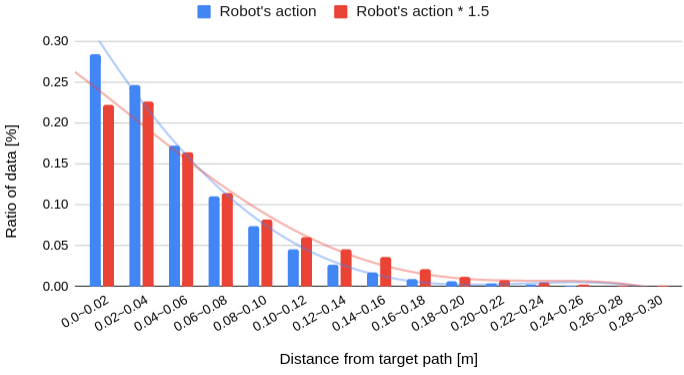
\includegraphics[keepaspectratio, scale=0.37]
        {images/hist_act_training2.png}
   \caption{Ratio of data by distance from target path in learning phase}
   \label{Fig:hist_act_training}
  \end{figure}  

  % \newpage

  テストフェーズにおける目標経路からの距離によるデータの割合を\figref{Fig:hist_act_test}に示す. この図から, 学習器から得られた角速度を1.5倍にした場合, データの割合が目標経路付近では増加し, 目標経路から離れた場所では減少している. よって, アプローチ2を試みた結果, テストフェーズでは目標経路付近の行動が増えた. すなわち, アプローチ2を試みる前に比べ, より正確に経路追従行動を模倣している可能性が高い.

  \begin{figure}[hbtp]
    \centering
   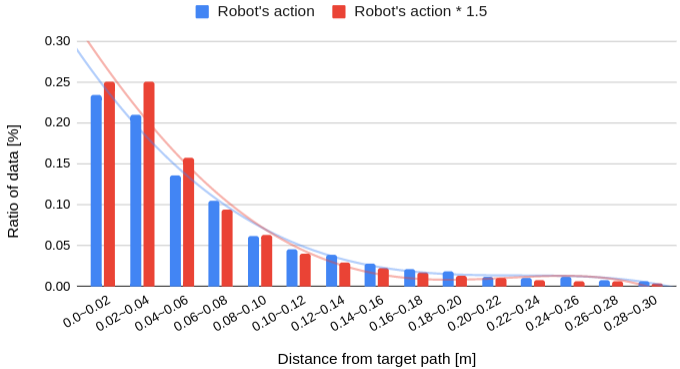
\includegraphics[keepaspectratio, scale=0.37]
        {images/hist_act_test2.png}
   \caption{Ratio of data by distance from target path in test phase}
   \label{Fig:hist_act_test}
  \end{figure}  

  % \newpage

% \end{itemize}

アプローチ1,2の実験を基に, 単に10000stepから20000stepに学習量を増やし, 実験した結果を下記に示す.

\figref{Fig:20000step_act1.5}は, それぞれの走行パターンにおいて正しく経路を選択し, 走行できた回数を表している. \tabref{table:result5} に実験ごとに全パターンの成功回数を合計した結果を示す. \tabref{table:result5} に示すように, 目標方向に従って 114/120 回, 正しい経路を選択する様子が見られた. また, 成功率が60000stepの実験と同程度になった. このことから, 2つのアプローチによって学習量が約67\%削減できたといえる.

\begin{figure}[hbtp]
  \centering
 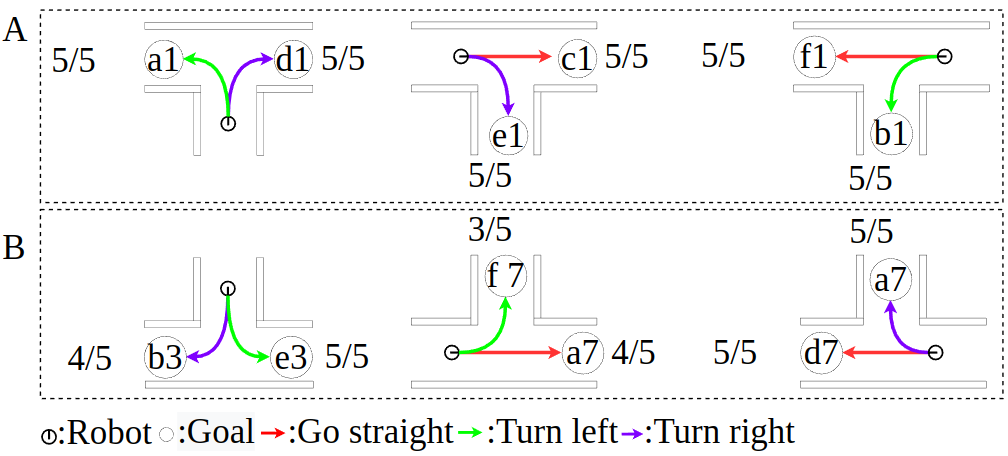
\includegraphics[keepaspectratio, scale=0.42]
      {images/20000step_act1.5.png}
 \caption{Experimental results for each moving pattern at 20000step by Approach 1+2}
 \label{Fig:20000step_act1.5}
\end{figure} 

\begin{table}[hbtp]
  \caption{Experimental results at 20000step by Approach 1+2}
  \label{table:result5}
  \centering
  \begin{tabular}{|c|c|c|}
    \hline
    Experiments & Step & Total results\\
    \hline
    Conventional & 60000 & 113/120(94.2\%)\\
    \hline
    Conventional & 10000 & 87/120(72.5\%)\\
    \hline
    Approach1:percentage change of data & 10000 & 99/120(82.5\%)\\
    \hline
    \begin{tabular}{c}
      Approach1:percentage change of data\\
      + Approach2:aggressive meandering
    \end{tabular} & 10000 & 109/120(90.8\%)\\
    \hline
    \begin{tabular}{c}
      \textbf{Approach1:percentage change of data}\\
      % \textbf{+}
      \textbf{+ Approach2:aggressive meandering}
    \end{tabular} & \textbf{20000} & \textbf{114/120(95\%)}\\
    \hline
  \end{tabular}
\end{table}

\newpage
